\documentclass{article}

% if you need to pass options to natbib, use, e.g.:
%     \PassOptionsToPackage{numbers, compress}{natbib}
% before loading neurips_2020

% ready for submission
% \usepackage{neurips_2020}

% to compile a preprint version, e.g., for submission to arXiv, add add the
% [preprint] option:
%     \usepackage[preprint]{neurips_2020}

% to compile a camera-ready version, add the [final] option, e.g.:
%	\usepackage[final]{neurips_2020}

% to avoid loading the natbib package, add option nonatbib:
%	\usepackage[nonatbib]{neurips_2020}
\usepackage[final, nonatbib]{neurips_2020}

\usepackage[utf8]{inputenc} % allow utf-8 input
\usepackage[T1]{fontenc}    % use 8-bit T1 fonts
\usepackage[hidelinks]{hyperref}       % hyperlinks
\usepackage{url}            % simple URL typesetting
\usepackage{booktabs}       % professional-quality tables
\usepackage{amsfonts}       % blackboard math symbols
\usepackage{amsmath}
\usepackage{nicefrac}       % compact symbols for 1/2, etc.
\usepackage{microtype}      % microtypography
\usepackage{multicol}
\usepackage{graphicx}
\usepackage{caption}
\usepackage{subcaption}

\title{Structural Compression of ResNet-like Convolutional Neural Networks using Separable Convolutions}

% The \author macro works with any number of authors. There are two commands
% used to separate the names and addresses of multiple authors: \And and \AND.
%
% Using \And between authors leaves it to LaTeX to determine where to break the
% lines. Using \AND forces a line break at that point. So, if LaTeX puts 3 of 4
% authors names on the first line, and the last on the second line, try using
% \AND instead of \And before the third author name.

\author{%
	Nicholas~Kastanos (nk569), Queens' College \\
	Department of Computer Science and Technology\\
	University of Cambridge\\
	Cambridge, CB3 0FD\\
	\texttt{nk569@cam.ac.uk} \\
}

\begin{document}
	
	\maketitle
	
	\begin{abstract}
		Convolutional neural networks (CNNs) are commonly used in computer vision neural networks, however inference on very deep models is resource intensive. In order to apply these CNNs to resource constrained devices, models must be compressed. By replacing convolution layers with separable convolutions, the number of parameters and multiply-accumulate operations can be reduced at the cost of performance. In this report, the compressibility of ResNet50V2 CNN model is investigated by replacing convolutions with spatial and depthwise convolutions. Additionally, the effects of 8-bit quantized compression on these layers is investigated. It is shown that a 8-bit compressed ResNet50V2 model with depthwise convolutions has a compression factor of $0.15$ while only experiencing a $1.34~\%$ decrease in accuracy.
	\end{abstract}
	
	\section{Introduction}
	
	Much of the research into convolutional neural networks (CNNs) is focused around increasing the performance of architectures for computer vision tasks, most commonly image classification and object detection \cite{resnetv1, vgg, yolo, inception, adscnet}. The applications of these neural networks, however, require efficient distributed training, fast inference times, and deployment to resource constrained hardware \cite{scalable8bit,mobilenet}. 
	
	Newer networks such as MobileNet \cite{mobilenet}, ShuffleNet \cite{shufflenet}, and EffNet \cite{effnet} each use different forms of separable convolutions to reduce the number of parameters and multiply-accumulate operations (MACs), while maintaining model performance. This structural compression allows CNNs to be applied to previously unavailable applications, such as autonomous vehicles, cellphones, and robotics.	While the benefits of separable convolutions can be seen in the networks which implement them, many other structural changes are also introduced. Therefore, the precise impact of separable convolutions ambiguous.
	
	In this paper, the effects of two types of separable convolutions -- spatial and depthwise -- are investigated in the ResNet50V2 architecture \cite{resnetv2}. This is achieved by replacing convolutional layers with separable variants, while making no other structural changes. Additionally, the effects of 8-bit quantization on the separable convolutions are investigated. Section~\ref{sec:background} gives contextual information on the CNN architecture and optimizations. The experiments use the TensorFlow framework \cite{tensorflow2015-whitepaper} for training and evaluation. Section~\ref{sec:methodology} details the experiment setup, while Section~\ref{sec:results} contains the experiment results and discussion. The source code used for the development of the neural networks can be accessed at \url{https://github.com/Nicholas-Kastanos/tf-cnn-compress}.
		
	% objectives and purpose
	
	\section{Related Work}
	\label{sec:background}
	%reasons behind work	
	% can discuss relationships between existing knowledge and what is being done here	
	\subsection{Residual networks}
	
	The residual block first postulated for use in ResNet has become a common-place feature in many subsequent networks \cite{resnetv1,inception,densenet}. It was designed to combat network degradation in very deep CNNs, where more complicated features were being learned than were required. The skip connections introduced by the residual block allow features to bypass convolutional blocks and be passed on to subsequent layers unaltered. This can be summarised in the formula $g(x) = f(x) + x$ where $x$ is the input, $g(x)$ is the desired output, and $f(x)$ is the input affected by the convolutional block.
	
	\begin{figure}[t!]
		\centering
		\begin{subfigure}[b]{\textwidth}
			\centering
			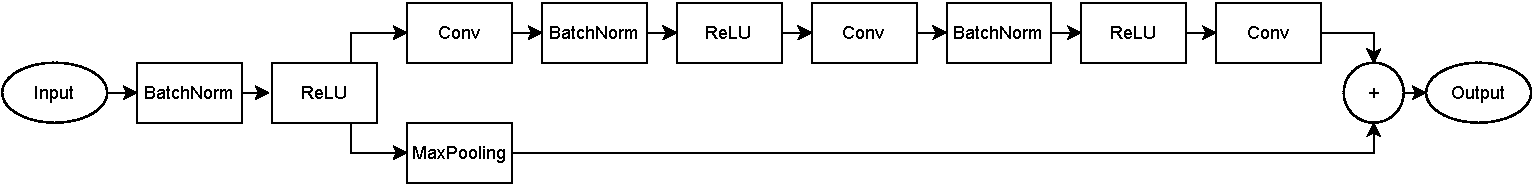
\includegraphics[width=\textwidth]{images/identity_base.pdf}
			\caption{Identity passthrough}
			\label{fig:resnet-identity}
		\end{subfigure}
		\vfill
		\begin{subfigure}[b]{\textwidth}
			\centering
			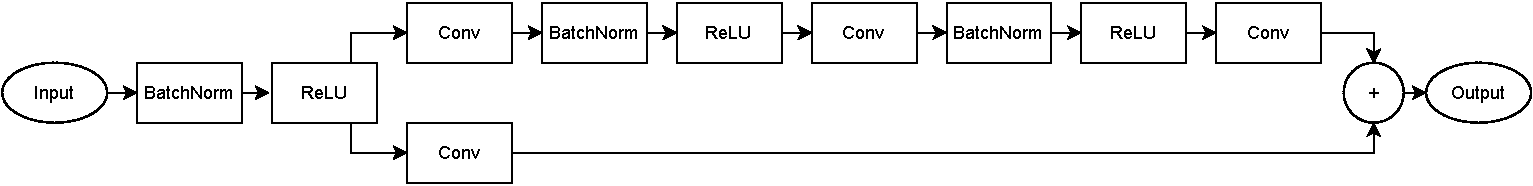
\includegraphics[width=\textwidth]{images/bottleneck_base.pdf}
			\caption{Bottleneck passthrough}
			\label{fig:resnet-bottleneck}
		\end{subfigure}
		\caption{Residual blocks used in ResNetV2}
		\label{fig:resnet}
	\end{figure}
	
	This architecture was further developed until the form presented in ResNetV2 \cite{resnetv2}, which includes two variants: identity passthrough which applies pooling to the skip connection $x$; and bottleneck passthrough, which includes a single convolution in the skip connection. These two residual blocks can be seen in Figure~\ref{fig:resnet}.
	
	\subsection{Separable convolutions}
	
	Convolution layers contain a vast majority of the parameters in modern CNNs \cite{inception,mobilenet,resnetv2}. By targeting parameter reductions to these layers, the compression can be spread throughout the network. Separable convolutions reduce the number of parameters by decomposing the convolution into multiple stages through spatially and depthwise separable convolutions. While these convolutions reduce the memory and computation requirements of the system, the reduced parameters limits the number of possible kernels explored in training, and the resulting network may be suboptimal.
	
	\subsubsection{Spatially separable convolutions}
	
	A convolution kernel can be decomposed on its 2D spatial axis, i.e. height and width \cite{inception,adscnet,effnet,squeezenet}. Conceptually, a $n \times n$ kernel can be separated into two smaller kernels, a $n \times 1$ followed by a $1 \times n$ kernel. These kernels can be applied in sequential convolutions to obtain the same output shape as the single convolution. These decomposed kernels scale the parameters required by the convolution by a factor $P_s(n)$ (see Equation~\ref{eqn:spat_params}). Similarly, the MAC operations of a spatially separated convolution are reduced. For a $N \times N$ input convolved with a $n \times n$ kernel, the number of multiplications are reduced by a factor of $M_s(n)$ (see Equation~\ref{eqn:spat_ops}). 
	
	Equations~\ref{eqn:spat_params})~and~\ref{eqn:spat_ops} show that spatially separable convolutions show computational benefits when $n > 2$. 
	
	\vspace{-1cm}
	
	\begin{multicols}{2}
		\begin{equation}\label{eqn:spat_params}
			P_s(n) = \frac{2}{n}
		\end{equation}
	\break
		\begin{equation}\label{eqn:spat_ops}
			\begin{split}
				M_s(N, n) = & \frac{2}{n} + \frac{2}{n(N-2)} \\
				\Rightarrow M_s(n) = & \frac{2}{n},~\text{where}~N >> n
			\end{split}
		\end{equation}		
	\end{multicols}
	
	\subsubsection{Depthwise separable convolutions}	
	
	Depthwise separable convolutions separate the spatial convolution from the depth of the filters \cite{mobilenet,xception}. This is accomplished by an initial depthwise convolution, followed by a pointwise convolution. The initial depthwise convolution separates the channels of the input and kernel, and convolves them independently. The pointwise convolution is a $N_F \times 1 \times 1 \times N_C$ convolution where $N_F$ and $N_C$ are the number of filters and channels respectively. 
	
	The number of parameters $P_d(n)$ and multiplications $M_d(n)$ are reduced by the same factor, which can be seen in Equation~\ref{eqn:depthwise}. Many CNNs have $N_F >> 1$, therefore depthwise convolutions show compression kernel sizes greater than 1  \cite{vgg, yolo, resnetv2}. 

	\begin{equation} \label{eqn:depthwise}
		P_d(n) = M_d(n) = \frac{1}{n^2} + \frac{1}{N_F} \approx \frac{1}{n^2}
	\end{equation}
	
%	\subsection{Quantised Training} I dont know if I want to do this anymore. Maybe just post trainng quantization
	
	\subsection{Quantization and datatype compression}
	
	Many resource-constrained devices do not have sufficient memory to use large neural networks, or may not have access to floating-point arithmetic units. Both of these factors can be mitigated by using low-precision integer datatypes, such as 8-bit integers \cite{scalable8bit,quantfriendlymobilenet}. This effectively reduces the memory required for each parameter by \nicefrac{1}{4}. However, by reducing the precision of the datatype, the learned parameters are not represented fully, reducing the performance of the network. This has been shown to have significant effect on the network when reducing 32-bit floating point numbers to 8-bit integers, however quantization aware training can limit the impact \cite{scalable8bit}. 
	
	TensorFlow, by default, uses 32-bit floating point precision for its network layers and training \cite{tensorflow2015-whitepaper}. TensorFlow Lite provides functionality to convert trained models to quantized, 8-bit integer models, however it does not have native 8-bit implementations for all layer types. In the event an incompatible layer is used, the engine upscales the activations to the full precision for that layer.
	
	\section{Methodology}
	\label{sec:methodology}
	% Use ResNet50V2
	In order to asses the benefits and costs of the compression, a baseline architecture is established and used as a reference point. The ResNet50V2 image classification CNN-based neural network is used as the baseline architecture. The baseline architecture and subsequent networks are trained using the same parameters. 
	
	\subsection{Training}
	%% how were the networks trained
	
	% Use of datasets CIFAR10
	The CNNs are trained using the CIFAR-10 dataset \cite{cifar10} in batches of 32, with random horizontal flips, rotations, and cropping data augmentations. The Adam optimizer \cite{adam} is used with a learning rate of $0.001$, and categorical crossentropy loss. The CIFAR-10 training split is separated into train and validation splits. The splits are not shuffled to ensure each model is trained on the same train and validation datasets, and the validation split contains $10\%$ of the total training data. The dataset's test split is used to evaluate the models on new data. The networks are trained until no improvement in the validation loss has been observed for $10$ epochs, at which point the best results weights are saved. This ensures that each model has enough time to learn its optimal weights.
	
	\subsection{Modified residual blocks}
	
	\begin{figure}[t!]
		\centering
		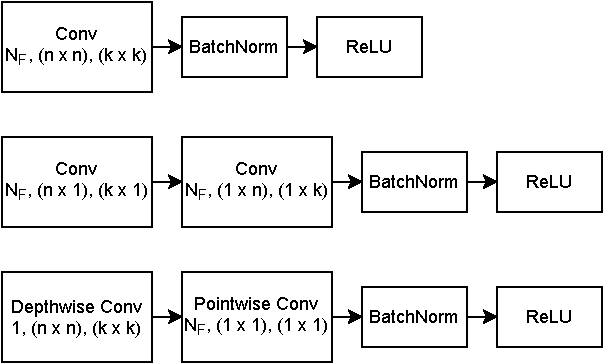
\includegraphics[width=0.5\textwidth]{images/conv-structure.pdf}
		\caption{Example of replaced convolutions with separable convolutions with $N_F$ filters, kernel size $n$, and stride $k$. From top to bottom: Traditional Convolution; Spatially Separable Convolution; Depthwise Separable Convolution}
		\label{fig:conv-structure}
	\end{figure}
	
		% How were convolutions separated / chosen for separation
	In order to modify the ResNetV2 network, the convolutions in the residual blocks are chosen to be substituted with separable convolutions. Additional batch normalization and activation layers are not added between these new layers. An example of this expansion can be seen in Figure~\ref{fig:conv-structure}. Only convolutions which would provide parameter and compute reduction are replaced with separable convolutions. For ResNet50V2, these are any convolutions where the kernel size $n > 1$. 
	
	\subsection{Post-training quantization and compression}
	% How were layers quantized
	The fully trained models are compressed to 8-bit precision using TensorFlow Lite. The framework recommends the provision of the representative dataset to enhance the optimization process. This allows for quantization of both weights and activations for quantizable operations. The representative dataset is compiled using 1000 samples from the training dataset. 	
	
	
	\section{Results and evaluation}
	\label{sec:results}
	
	The trained CNNs are evaluated using the test split of CIFAR-10. The dataset includes 1000 samples from each of the 10 classes, ensuring class balance. The models are evaluated by creating TensorFlow Lite models from the original model. In the case of compressed models, the TensorFlow Lite model converter optimizes the models and quantises the activations using the representative dataset. 
	
	Table~\ref{tbl:params} shows the total parameters in the ResNet50V2 models. This shows that substituting separable convolutions into a CNN, the total number of parameters can be reduced by up to $57~\%$. Table~\ref{tbl:params} also shows training performance of the models.
	
	\begin{table}[b!]
		\caption{Training statistics}
		\label{tbl:params}
		\centering
		\begin{tabular}{lllll}
			\toprule
			Convolution Type & Total Parameters & Best Epoch & Train Loss & Validation Loss \\ \midrule
			Full             & $23,585,290$     & 54         & 0.2539     & 0.2560          \\
			Spatial          & $19,812,874$     & 70         & 0.2478     & 0.2888          \\
			Depthwise        & $13,559,498$     & 47         & 0.4447     & 0.3516          \\ \bottomrule
		\end{tabular}
	\end{table}
	
	\begin{table}[b!]
		\caption{Results using the test split of CIFAR-10}
		\label{tbl:results}
		\centering
		\begin{tabular}{lllll}
			\toprule
			Convolution Type     & Loss     & Accuracy (\%)    & Size (kB) & Compression Factor \\ \midrule
			Full                 & $1.0045$ & $74.63$          & $94,145$  & $1$                \\
			Spatial              & $1.0334$ & $74.09$          & $79,064$  & $0.84$             \\
			Depthwise            & $0.8940$ & $73.38$          & $54,050$  & $0.57$             \\
			Compressed Full      & $1.3332$ & $73.99$          & $24,446$  & $0.26$             \\
			Compressed Spatial   & $1.4457$ & $73.61$          & $20,770$  & $0.22$             \\
			Compressed Depthwise & $1.0686$ & $\mathbf{73.29}$ & $14,517$  & $\mathbf{0.15}$    \\ \bottomrule
		\end{tabular}
	\end{table}

	Table~\ref{tbl:results} shows the results of the analysis. The compression factor is the ratio of the model size under investigation to that of the ResNet50V2 baseline model. As seen in Table~\ref{tbl:results}, applying spatial convolutions to ResNet50V2 has a compression factor of $0.84$ while the drop in accuracy is $0.54~\%$. Depthwise convolutions result in an accuracy drop of $1.25~\%$ while compressing the network with compression factor of $0.57$.
	
	Applying both depthwise convolution substitution and 8-bit quantized compression results in a model approx 6.5 times smaller than the full ResNet50V2 model. This model does not significantly impact the performance of the model as seen by the accuracy decreasing by only $1.34~\%$. In addition to storage size, the maximum RAM requirements can be analysed by \verb|tflite-tools| \cite{tflietools}. The uncompressed models require a maximum of $196.61~kB$, while the compressed versions require $49.15~kB$. This memory requirement is constant across convolution types because the most memory intensive layers of ResNet50V2 are input processing layers.
	
	% include implications of results
	The significant reduction in parameters and memory improvements shown by separable convolutions with very small drawbacks allows complicated CNN networks to be implemented on resource constrained devices. This is especially true for larger CNNs such as ResNet152V2 or YOLO object detection networks, as they are too large to operate uncompressed on MCU or FPGA devices. Efficient computer vision CNNs can be used to operate self-driving vehicles, drones, and other robotics. This allows the applications to be smaller, and more energy efficient, allowing for more possible applications. 
	
	%Limitations
	Large benefits are observed for ResNet50V2, however, these benefits are not without limits. The separable convolutions were only applied to $3 \times 3$ kernels, as ResNet does not include larger kernel sizes on a regular basis. While Equations~\ref{eqn:spat_params},~\ref{eqn:spat_ops},~and~\ref{eqn:depthwise} show that the compressive benefits of separable convolutions increase with kernel size, so too does the degradation in performance. This performance loss is not quantified by the results seen in Table~\ref{tbl:results}.
	
	\section{Future Work}
	
%	Larger kernels
	In order to determine the validity of separable convolutions for larger networks, further investigation into larger kernel and input sizes is required. If these convolution decompositions do not result in significant performance degradations, further improvements to CNN compression can be observed.

%	Combining depth and spatial
	The initial depthwise convolution is $n \times n$, which can be separated spatially. The combination of these two techniques can result in further optimisation.
	
	% Quantized Training
	
	\section{Conclusion}
	
	ResNet-like neural networks are common in image applications, however their large size and complexity prevents them from being used in resource constrained scenarios. By replacing the convolution layers with spatially and depthwise separable convolutions, the memory and compute intensive convolutional layers can be compressed. These separable convolution layers were applied to the ResNet50V2 image classification CNN trained on the CIFAR-10 dataset, along with 8-bit quantization. The resulting network has a compression factor of $0.15$ while only observing a $1.34~\%$ decrease in accuracy. The now compressed network can be deployed to resource constrained devices to classify images at high accuracy while maintaining a low computational overhead.
	
	\newpage
	\bibliographystyle{ieeetr}
	\bibliography{references}
	
\end{document}